\section{Appendix}

\appendix


\section{Disentangling token and positional signal in the output of S-Inhibition Heads} \label{app:disantangling_signals}

In Section \ref{sec:s_inhibition}, we discovered that S-Inhibition Heads are responsible for the Name Mover Heads' specific attention on the IO token, and in particular we discovered that their output is a signal for Name Movers Heads to avoid the S1 token. 

More precisely, we discover that they were outputting \emph{token signals} (information about the value of the token S) and \emph{positional signals} (related to the value of the position S1). We describe here the details of this discovery.

To disentangle the two effects, we design a series of counterfactual datasets where only some signals are present, and some are inverted with respect to the original dataset. In this section, we conducted activation patching (or simply patching). Instead of patching isolated paths, we patch the output of a set of heads and recompute the forward pass of the model after this modification. As shown in Section \ref{sec:distributed_name_movers}, the output of later (Backup) Name Mover Heads and Negative Heads depend on earlier heads from these classes, such that it is not possible to ignore the interactions between heads inside a class (as it is the case in path patching in Appendix \ref{app:path_patching}).

By patching the output of S-Inhibition heads from these datasets, we can quantify in isolation the impact of each signal on the final logit difference.

We constructed six datasets by combining three transformations of the original $\pioi$ distribution.
\begin{compactitem}
    \item \textbf{Random name flip}: we replace the names from a given sentence with random names, but we keep the same position for all names. Moreover, each occurrence of a name in the original sentence is replaced by the same random name. When we patch outputs of S-Inhibition heads from this sentence, only positional signals are present, the token signals are unrelated to the names of the original sequence.
    \item \textbf{IO$\leftrightarrow$S1 flip}: we swap the position of IO and S1. The output of S-inhibition heads will contain correct token signals (the subject of the second clause is the same) but inverted positional signals (because the position of IO and S1 are swapped)
    \item \textbf{IO$\leftarrow$S2 replacement}: we make IO become the subject of the sentence and S the indirect object. In this dataset, both token signals and positional signals are inverted.
\end{compactitem}
We can also compose these transformations. For instance, we can create a dataset with no token signals and inverted positional signals by applying IO$\leftrightarrow$S1 flip on the dataset with random names. In total, we can create all six combinations of original, inverted, or uncorrelated token signal with the original and inverted positional signal.

From each of those six datasets, we patched the output of S-Inhibition heads and measured the logit difference. The results are presented in Figure \ref{table:signals_logit_diff}.



\begin{figure}
\begin{center}
\begin{tabular}{ |c|c|c|c|} 
\hline
\textbf{~} & \textbf{Original positional signal} & \textbf{Inverted position signal} \\ 
\hline 
Original S token signal & 3.55 (baseline) & -0.99  \\
\hline
Random S token signal& 2.45 & -1.96  \\
\hline
S$\leftrightarrow$IO inverted token signal & 1.77 & -3.16  \\
\hline
\end{tabular}
\caption{Logit difference after patching S-Inhibition heads from signal-specific datasets. The effect on logit difference can be decomposed as a sum of the effects of position and token signal. }
\label{table:signals_logit_diff}
\end{center}
\end{figure}

\begin{figure}
    \centering

     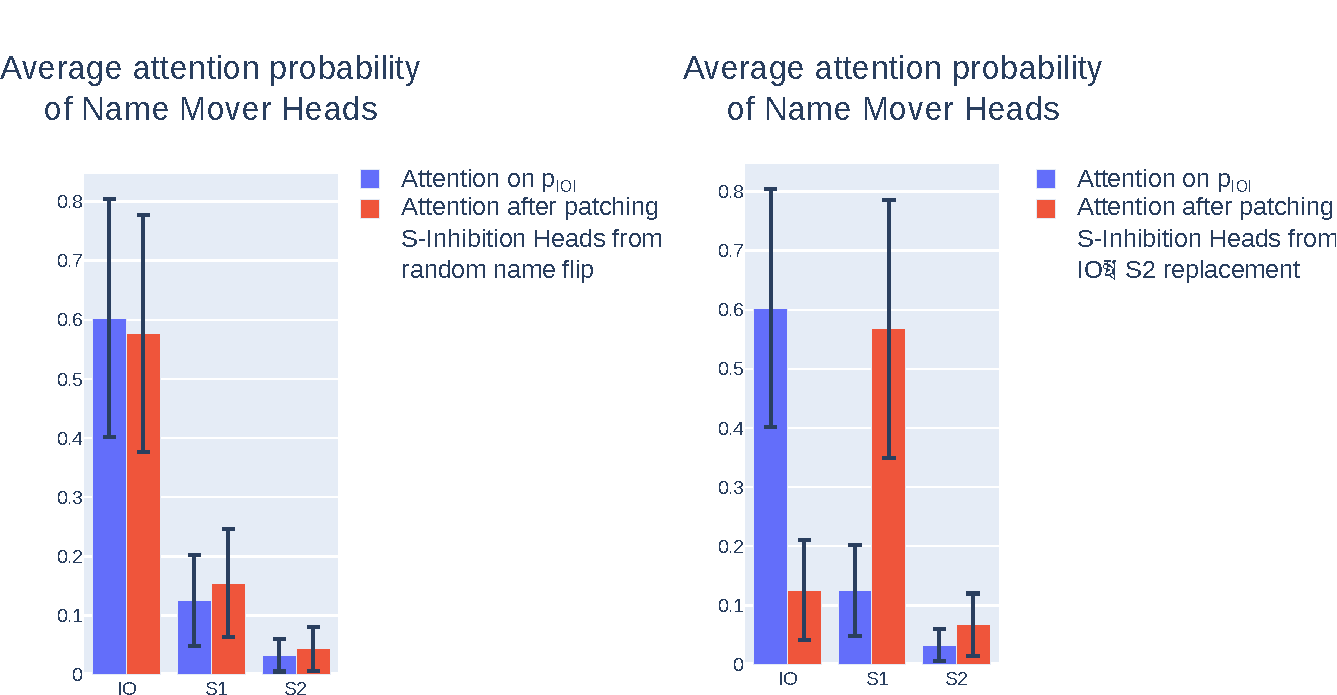
\includegraphics[width=0.7\textwidth]{figs/sin_s2_replacement_nm_attention.pdf}

    \caption{Name Mover Heads' attention probability before and after patching S-Inhibition Heads from signal-specific datasets. Left: patching from the dataset generated by random flip of name (same position signal, random token signal). Right: patching from the dataset generated by IO$\leftarrow$S2 replacement (inverted position signal, inverted token signal). Black bars represent the standard deviation.   }
    \label{fig:effect_s_in_patching_nm_attention}
\end{figure}

These results can be summarized as the sum of the two effects. Suppose we define the variable $S_{tok}$ to be 1 if the token signal is the original, 0 when uncorrelated and -1 when inverted. And similarly $S_{pos}$ to be 1 if the position signal is the original and -1 if inverted. Then the Figure \ref{table:signals_logit_diff} suggests that the logit difference can be well approximated by $2.31S_{pos} + 0.99S_{tok}$, with a mean error of 7\% relative to the baseline logit difference.

For instance, when both the positional and token signals are inverted, the logit difference is the opposite of the baseline. This means that the S token is predicted stronger than the IO token, as strong as IO before patching. In this situation, due to the contradictory information contained in the output of S-Inhibition heads, the Name Movers attend and copy the S1 token instead of the IO token (see Figure \ref{fig:effect_s_in_patching_nm_attention}, right). 
In the intermediate cases where only one of the signals is modified, we observe a partial effect compared to the fully inverted case (e.g. Figure \ref{fig:effect_s_in_patching_nm_attention}, left). The effect size depends on the altered signals: positional signals are more important than token signals. 

Can we be more specific as to what the token and positional signals are? Unfortunately, we do not have a complete answer, but see this as one of the most interesting further directions of our work. We expect that the majority of the positional information is about the \emph{relative} positional embedding between S1 and S2 (such pointer arithmetic behavior has already been observed in \citet{olsson2022context}). When patching in S2 Inhibition outputs from a distribution where prefixes to sentences are longer (but the distance between S1 and S2 is constant), the logit difference doesn't change (3.56 before patching vs 3.57 after).  This suggests that the positional signal doesn't depend on the absolute position of the tokens, as long as the relative position of S1 and S2 stays the same.

% AC: comment out
% These results are incomplete and invite future work to thoroughly investigate this phenomenon. We suggest two main avenue for future work. First, what are exactly, positional signal? Preliminary results suggest that they are dependent on the distance between S1 and S2 \ac{would be great to add evidence}. This suggests that they encode for relative positional pointers like ``S1 is X tokens before'' in opposition to absolute position ``S1 is at position Y'' \ac{reword?}. The second direction is about the encoding of positional signal in the residual stream. We hypothesized that there could be an interaction with the space of positional embeddings.
% AC done



\section{Path patching}
\label{app:path_patching}

% In this section we describe the technical details of the path patching technique we used in many experiments.
% All path patching experiments have a set of sender heads and receiver model components.
% ``Receiver model components'' may be the logits, or the heads’ $Q$ values, $K$ values, or $V$ values.
% We use $\pioi$ as the input distribution for these experiments, but with the following modifications to the outputs of groups of heads:

% \begin{enumerate}
% \item We patch the sender heads’ output activations from the $\pabc$ distribution.
% \item We freeze the $Q$, $K$ and $V$ values of all heads to their $\pioi$ values, except for the sender heads and the receiver model components.
% \item We do not freeze the activations of the receiver model components.
% \end{enumerate}

% This attempts to measure the direct effect of the sender head on the receiver model components.
% However, we do not claim that this is a canonical choice. We’ve identified at least two limitations with this approach.

% Firstly, in this approach, receiver model components in later layers have inputs from earlier receiver model components with modified output. This means that this approach measures both the direct effect of the sender head on receiver model components, and the indirect inner interactions between receiver model components. Additionally, MLPs are never frozen or patched and hence also may cause indirect effects that are beyond the scope of this work.

\begin{figure}
    \centering
    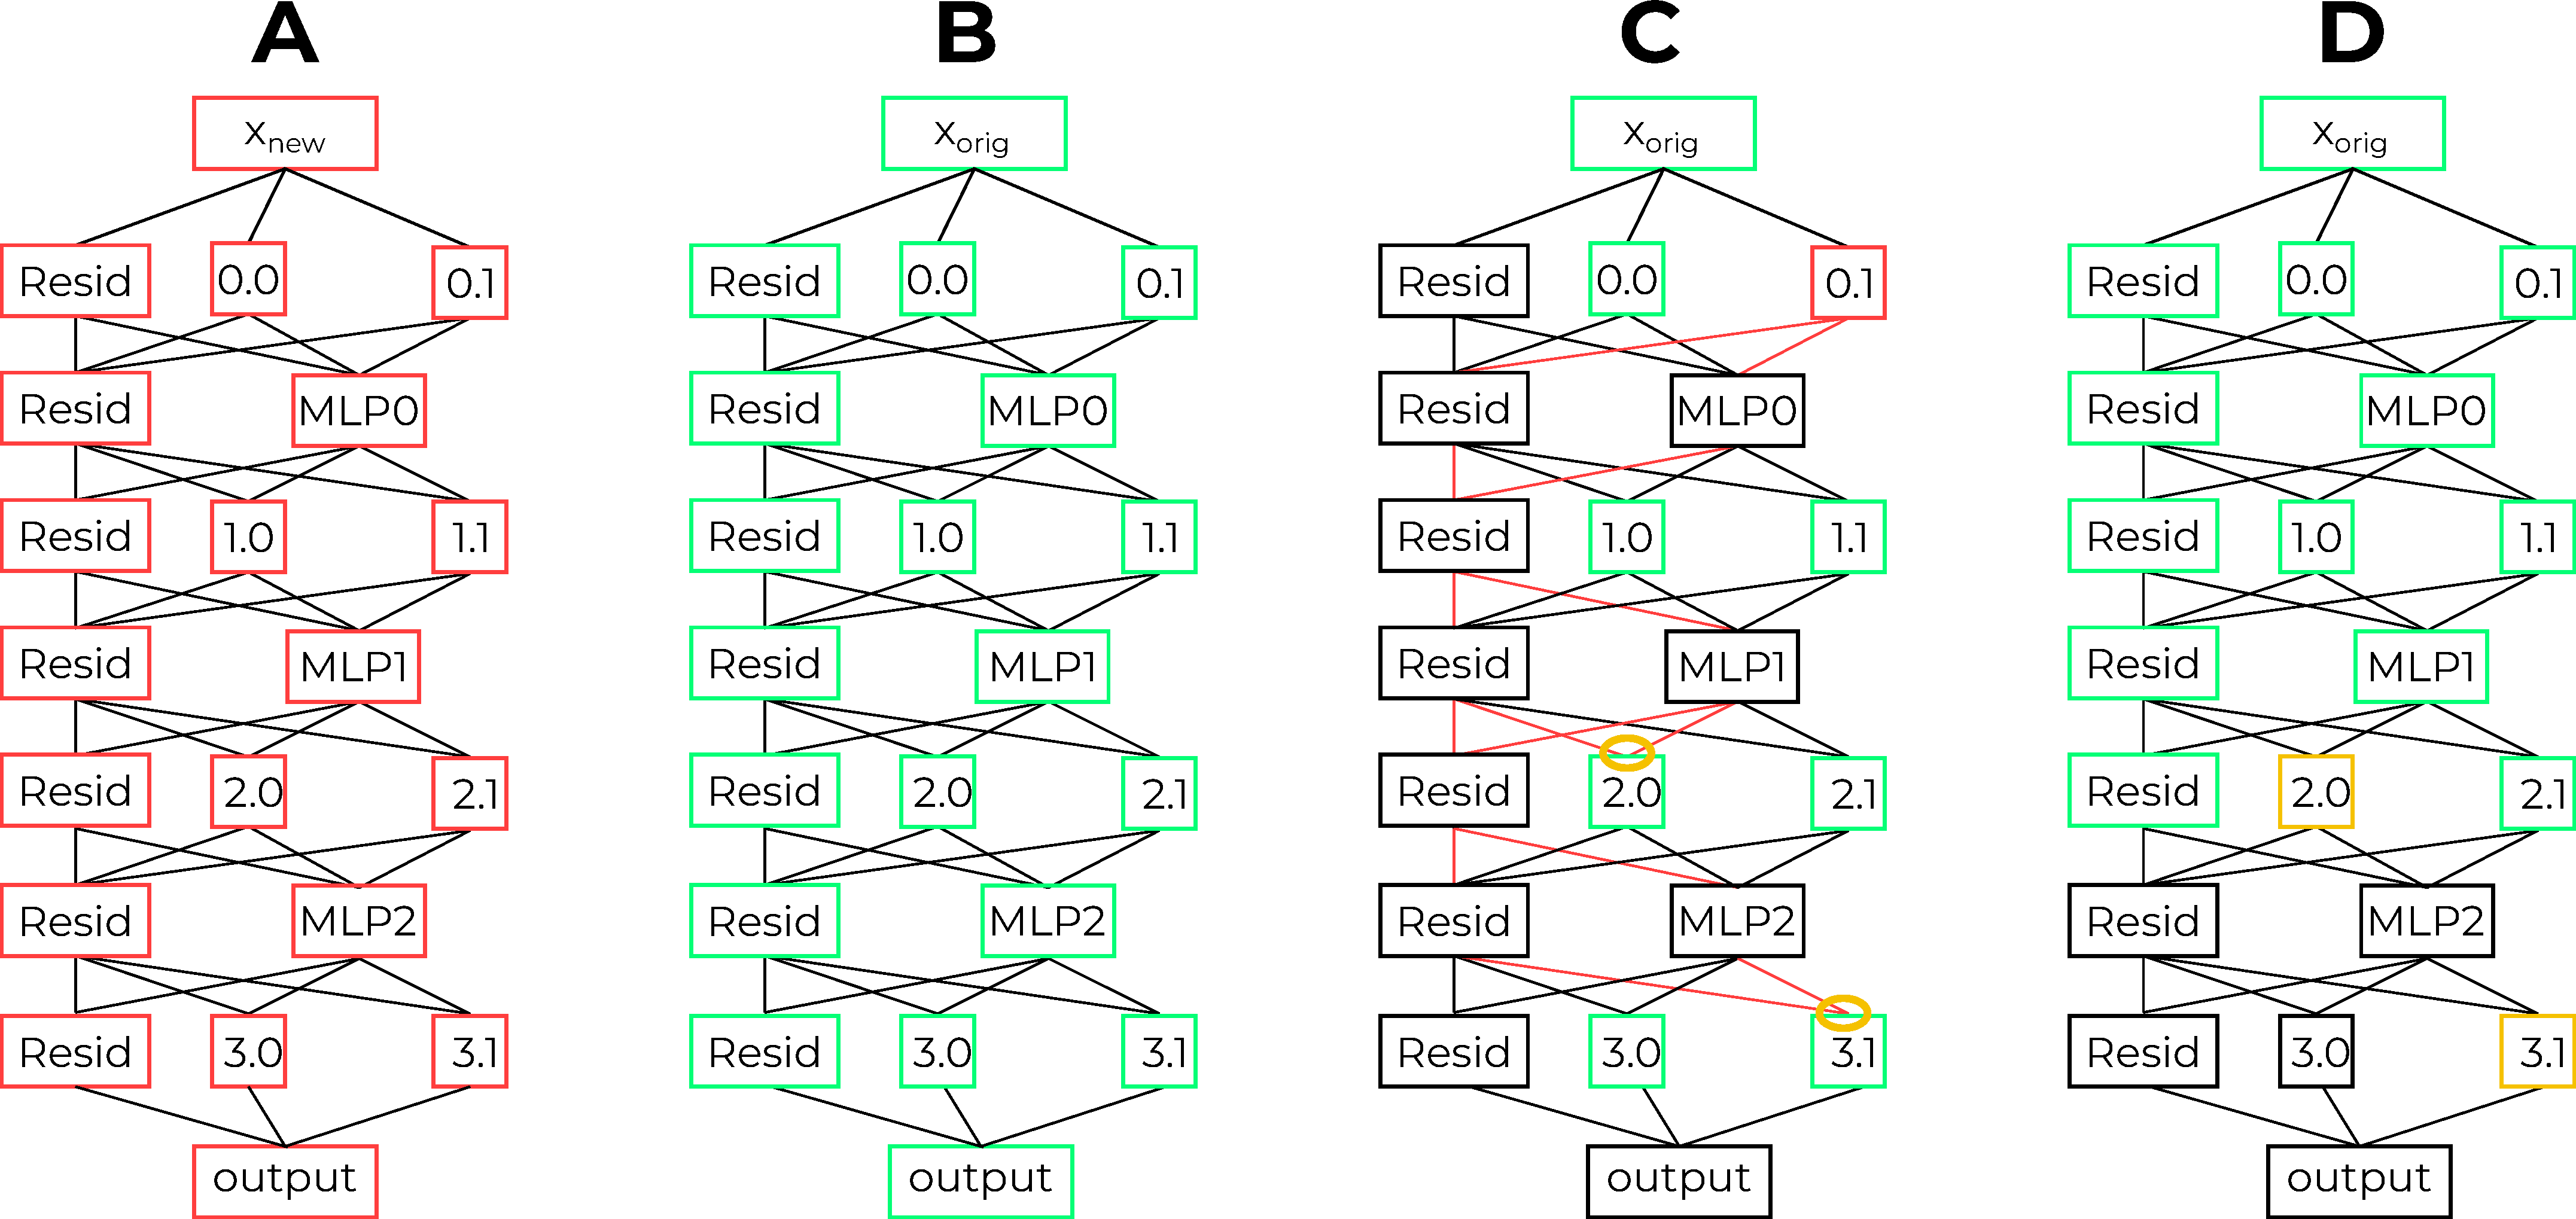
\includegraphics[width=\textwidth]{figs/path_patching.pdf}
    \caption{Illustration of the four forward passes in the path patching method. $h=0.1$ and $R=\{2.0, 3.1\}$. The layer norms are not shown for clarity. In the forward pass C, we show in red all the paths through which $h$ can influence the value of heads in $R$. Nodes in black are recomputed, nodes in color are patched or frozen to their corresponding values.}
    \label{fig:path_patching}
\end{figure}

In this section we describe the technical details of the path patching technique we used in many experiments. This technique depends on

\begin{itemize}
    \item $x_{\text{orig}}$ the original data point,
    \item $x_{\text{new}}$ the new data point,
    \item $h$ the \textit{sender} attention head, and
    \item $R \subseteq M$ the set of \textit{receiver} nodes in the model's computational graph $M$. In our case, $R$ is either the input (key, query or values) of a set of attention heads or the end state of the residual stream\footnote{The model uses the end state of the residual stream to compute the logits (after a layer norm), so we choose $R$ equal to this end state when we wish to measure the direct effect of $h$ on the logits.}.
\end{itemize}

It is then implemented as Algorithm \ref{path_patching}, which can be summarized in five steps.

\begin{enumerate}
    \item Gather activations on $x_{\text{orig}}$ and $x_{\text{new}}$. [Lines 1-2, Figure \ref{fig:path_patching}A-B]
    \item Freeze\footnote{We use `freezing' of an activation $a$ to refer to the special case of patching when we begin a forward pass on an input $x$, edit some earlier activations, and then want to patch $a$ to its value on a forward pass of $x$ (which did not have the edits of earlier activations).} all the heads to their activation on $x_{\text{orig}}$ except $h$ that is patched to its activation on $x_{\text{new}}$. [Lines 4-5, Figure \ref{fig:path_patching}C]
    \item Run a forward pass of the model on $x_{\text{orig}}$ with the frozen and patched nodes (MLPs and layer norm are recomputed). [Line 7, Figure \ref{fig:path_patching}C]
    \item In this forward pass, save the activation of the model components $r \in R$ as if they were recomputed (but this value is overwritten in the forward pass because they are frozen). [Line 6-9, Figure \ref{fig:path_patching}C]
    \item Run a last forward pass on $x_{\text{orig}}$ patching the receiver nodes in $R$ to the saved values. [Lines 12-20,  Figure \ref{fig:path_patching}D]
\end{enumerate}

Each of the $A$ variables in Algorithm \ref{path_patching} ($A_{\mathrm{orig}}$, $A_{\mathrm{new}}$ and $A_{\mathrm{patch}}$) stores activations for all nodes in $M$. $A_{\mathrm{orig}}$ and $A_{\mathrm{new}}$ contain output activations while $A_{\mathrm{patch}}$ contains the activation of the nodes in $R$ (keys, queries or values of attention heads, or the end state of the residual stream).

In forward pass C of the algorithm all attention heads except $h$ have their output frozen to their value on $x_{\text{orig}}$. This means that we remove the influence of every path including one (or more) intermediate attention heads $p$ of the form $h \to p \to r$, where $r \in R$. In all cases in the paper, we measure the logit difference on the forward pass D compared to the logit difference of the model, as a measure of the importance of the path $h \to r$. We additionally compute this logit difference as an average over $N>200$ pairs $(\xorig, \xnew)$.

% Note that in the case where we are interested in the direct influence on logits (as in Section \ref{sec:name movers}), we do not compute the forward pass D in Figure \ref{fig:path_patching}. Instead, in the forward pass C, we measure the output logits and stop here. 


\begin{algorithm}
\caption{Path patching}\label{path_patching}
\begin{algorithmic}[1]
% \Require Set of sender heads $S$, Set of receiver heads $R$, receiver heads' input $I\in \{Q,K,V\}$, model $M$, Original dataset $D_{\mathrm{orig}}$, New dataset $D_{\mathrm{new}}$; returns logits after path patching.
% \State $L \gets \mathrm{Max}_{h \in R}~layer(h)$ \Comment{\ac{isn't this min?}}
% \State $H \gets \text{All attention heads from $M$, with layer $\leq L$}$
\State Compute all activations $A_{\mathrm{new}}$ on $x_{\text{new}}$ (forward pass A)% \gets \text{Activation of $S$ from $M(D_{\mathrm{new}})$}$
\State Compute all activations $A_{\mathrm{orig}}$ on $x_{\text{orig}}$ (forward pass B)
\For{$r \in R$}
    \State $A^r_{\text{patch}} \gets A_{\mathrm{orig}}$
    \State $A^r_{\text{patch}}[h] \gets A^r_{\text{new}}[h]$
    \For{each MLP $m$ between $h$ and $r$}
        \State Recompute $A^r_{\text{patch}}[m]$ from the activations in $A^r_{\text{patch}}$ (forward pass C) % from $D_{\text{orig}}$, all earlier MLPs and attention heads in $A^r_{\text{patch}}$.
    \EndFor
    \State Recompute $A^r_{\text{patch}}[r]$ from the activations in $A^r_{\text{patch}}$ (forward pass C)
\EndFor\\

\State $A_{\text{final}} \gets \emptyset$
\For{$c \in M$ nodes of the computational graph, in topologically sorted order,} (forward pass D)
    \If{$c \in R$}
        \State $A_{\text{final}}[c] \gets A^c_{\text{patch}}[c] $
    
    \Else
        \State Compute $A_{\text{final}}[c]$ from activations in $A_{\text{final}}$ 
    \EndIf
\EndFor \\

% \State Recompute 
\Return $A_{\text{final}}[\text{Logits}]$ % Recomputation of logits from activations in $A^r_{\text{final}}$ (forward pass D)% $\mathrm{Logits} recomputed from % c\text{ from a forward pass on } D_{\text{new}} \text{ with all } r \in R\text{'s activations replaced by }A^r_{\text{patch}}[r]$
\end{algorithmic}
\end{algorithm}






\section{Direct effect on S-Inhibition Heads' keys} \label{app:s_in_keys}

In this section, we present the direct effect analysis of the S-Inhibition Heads' keys. The experiment is similar to the investigation of the S-Inhibition Heads' values presented in Section \ref{sec:s_inhibition}.

The results presented in Figure \ref{fig:effect_on_sin_keysB} show that some heads significantly influence the logit difference through S-Inhibition Heads' keys. We observe that Duplicate Token Heads (3.0 and 0.1) appear to also influence S-Inhibition Heads' values, but their effect is reversed.

Moreover, we identify 3 new heads influencing positively the logit difference: 5.9, 5.8 and 0.10. 

\textbf{Fuzzy Duplicate Token Head} By looking at its attention pattern, we identified that 0.10 was paying attention to S1 from S2. However, the attention pattern was fuzzy, as intermediate tokens also have non-negligible attention probability. We thus call it a fuzzy Duplicate Token Head. On Open Web Text (OWT), the fuzzy Duplicate Token Head attend to duplicates in a short range (see Appendix~\ref{app:validation_dups}).

\textbf{Fuzzy Induction Heads} The heads 5.9, 5.8 are paying attention to S1+1. For 5.8, S1+1 is the token with the highest attention probability after the start token. But the absolute value is small (less than 0.1). The head 5.9 is paying attention to S1+1 but also to tokens before S. Because of these less interpretable attention patterns, we called them fuzzy Induction Heads. (see Appendix~\ref{app:random_tok_seq} for more details about their behavior outside IOI).

By influencing the keys of the S-Inhibition Heads, we hypothesize that those heads are amplifying the positional signal written by the other Induction and Duplicate Token Heads.



\begin{figure}
    \centering
     \begin{subfigure}[b]{0.43\textwidth}
         \centering
         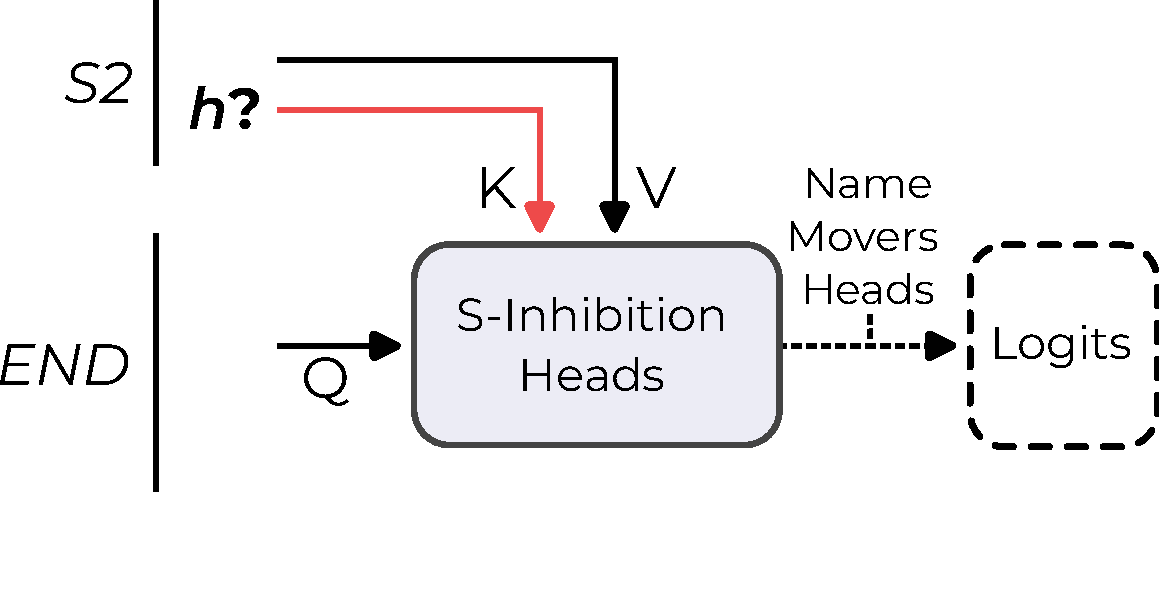
\includegraphics[width=\textwidth]{figs/Direct_effect_on_sin_keysA.pdf}
         \caption{}
         \label{fig:effect_on_sin_keysA}
     \end{subfigure}
     \hfill
     \begin{subfigure}[b]{0.43\textwidth}
         \centering
         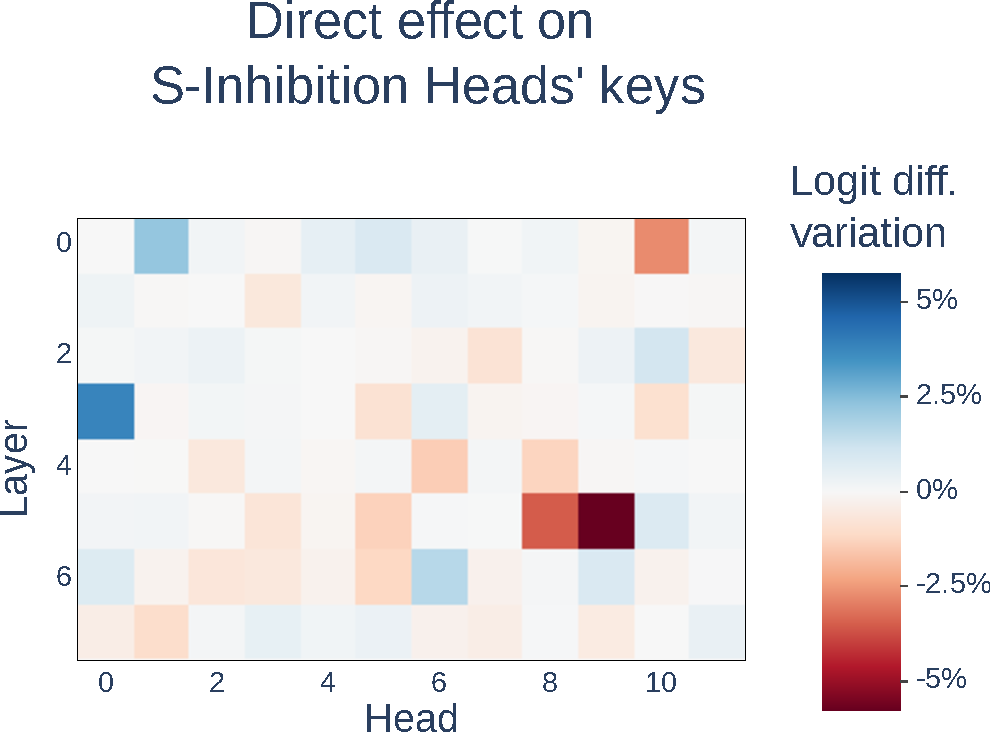
\includegraphics[width=\textwidth]{figs/Direct_effect_on_sin_keysB.pdf}
         \caption{}
         \label{fig:effect_on_sin_keysB}
     \end{subfigure}
    \caption{(a) Diagram of the direct effect experiment on S-Inhibition Heads' keys at S2. (b) Result of the path patching experiments for direct effect experiment on S-Inhibition Heads' keys.}
    \label{fig:effect_on_sin_keys}
\end{figure}

\section{Identification of Previous Token Heads} \label{app:prev_token_heads}

Induction Heads rely on key composition with Previous Token Heads to recognize patterns of the form \texttt{[A]\,[B]\,...\,[A]}. In the context of IOI, the repeated token \texttt{[A]} is S2. We thus searched for heads directly affecting Induction Heads keys at the S1+1 position (the \texttt{[B]} token in the general pattern). For this, we used path patching. The results of the experiment are visible in Figure \ref{fig:prev_tok}. We identify two main heads causing a decrease in logit difference (and thus contributing positively to the logit difference): 4.11 and 2.2. These heads pay primary attention to the previous token. This is coherent with the Previous Token Heads we were expecting. We thoroughly investigate their attention patterns outside of $\pioi$ in Appendix \ref{app:random_tok_seq}.

\citet{olsson2022context} also describes an induction mechanism relying on query composition in GPT-2. We performed path patching to investigate heads influencing the Induction Heads queries at the S2 position, but did not find any significant effect.

\begin{figure}
    \centering
     \begin{subfigure}[b]{0.43\textwidth}
         \centering
         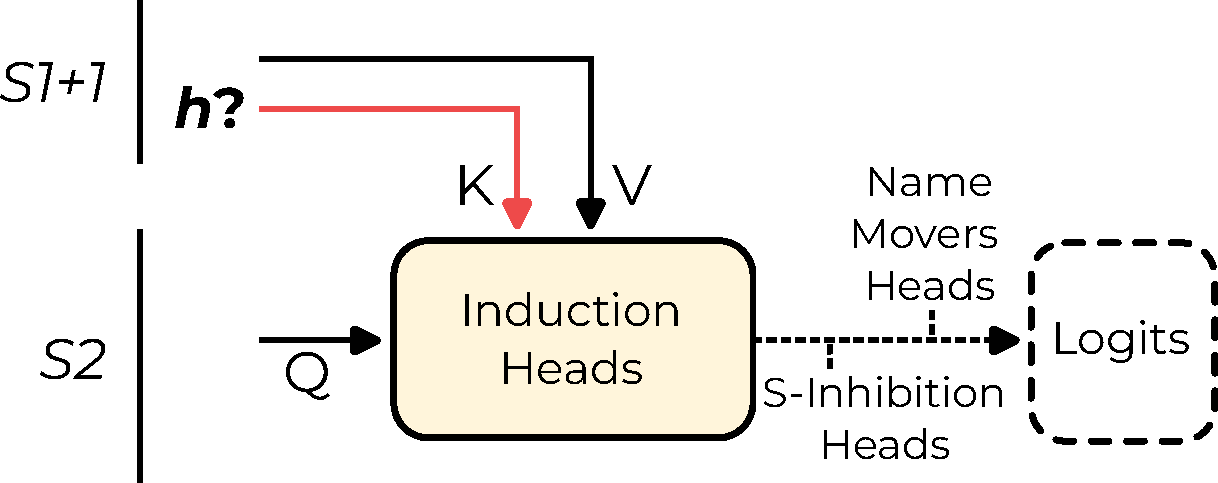
\includegraphics[width=\textwidth]{figs/prev_tokA.pdf}
         \caption{}
         \label{fig:prev_tokA}
     \end{subfigure}
     \hfill
     \begin{subfigure}[b]{0.43\textwidth}
         \centering
         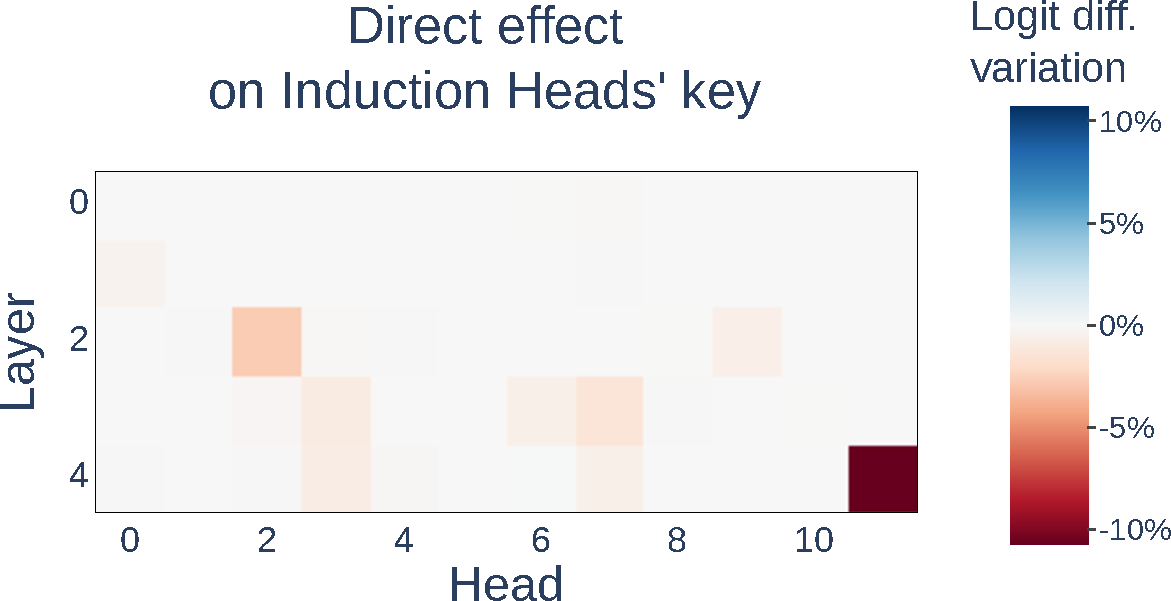
\includegraphics[width=\textwidth]{figs/prev_tokB.pdf}
         \caption{}
         \label{fig:prev_tokB}
     \end{subfigure}
    \caption{(a) Diagram of the direct effect experiment on Induction Heads' keys at S1+1. The effects on logits are mediated by S-Inhibition Heads and Name Mover Heads (b) Result of the path patching experiments on Induction Heads' keys at S1+1.}
    \label{fig:prev_tok}
\end{figure}

\section{IOI Templates} 
\label{app:templates}
We list all the templates we used in Figure \ref{fig:table_templates}. Each name was drawn from a list of 100 English first names, while the place and the object were chosen among a hand-made list of 20 common words. All the words chosen were one token long to ensure proper sequence alignment computation of the mean activations.

\begin{figure}[H]
\centering
\begin{tabular}{ |c| } 
\hline
Templates in $\pioi$ \\ 
\hline 
Then, [B] and [A] went to the [PLACE]. [B] gave a [OBJECT] to [A] \\
\hline
Then, [B] and [A] had a lot of fun at the [PLACE]. [B] gave a [OBJECT] to [A] \\
\hline
Then, [B] and [A] were working at the [PLACE]. [B] decided to give a [OBJECT] to [A] \\
\hline
Then, [B] and [A] were thinking about going to the [PLACE]. [B] wanted to give a [OBJECT] to [A] \\
\hline
Then, [B] and [A] had a long argument, and afterwards [B] said to [A] \\
\hline

After [B] and [A] went to the [PLACE], [B] gave a [OBJECT] to [A] \\
\hline

When [B] and [A] got a [OBJECT] at the [PLACE], [B] decided to give it to [A] \\
\hline

When [B] and [A] got a [OBJECT] at the [PLACE], [B] decided to give the [OBJECT] to [A] \\
\hline

While [B] and [A] were working at the [PLACE], [B] gave a [OBJECT] to [A] \\
\hline
While [B] and [A] were commuting to the [PLACE], [B] gave a [OBJECT] to [A] \\
\hline
After the lunch, [B] and [A] went to the [PLACE]. [B] gave a [OBJECT] to [A] \\
\hline
Afterwards, [B] and [A] went to the [PLACE]. [B] gave a [OBJECT] to [A] \\
\hline

Then, [B] and [A] had a long argument. Afterwards [B] said to [A] \\
\hline

The [PLACE] [B] and [A] went to had a [OBJECT]. [B] gave it to [A] \\
\hline

Friends [B] and [A] found a [OBJECT] at the [PLACE]. [B] gave it to [A] \\
\hline
\end{tabular}
\caption{Templates used in the IOI dataset. All templates in the table fit the `BABA' pattern, but we use templates that fit the `ABBA' pattern as well (i.e, by swapping the first instances of [B] and [A] in all of the above).}
\label{fig:table_templates}
\end{figure}

\section{Backup Name Mover Heads} \label{app:backup_name_movers}

Here we discuss in more detail the discovery of the Backup Name Mover Heads. As shown in Figure \ref{fig:backup_nm_discovery}, knocking-out the three main Name Mover Heads surprisingly changes the behavior of the other heads that write in the IO-S direction (both positively and negatively). These heads compensate for the loss of function from the Name Mover Heads such that the logit difference is only 5\% lower. We observe that the Negative Name Mover Heads have a less negative effect on logit difference, and 10.7 even has a positive effect on the logit difference after the knockout. The other heads that affected slightly positively the logit difference before the knock-out become the main contributors. Both the reason and the mechanism of this compensation effect are still unclear. We think that this could be an interesting phenomenon to investigate in future works.

Among the heads influencing positively the logit difference after knockout, we identified S-Inhibition Heads and a set of other heads that we called \emph{Backup Name Mover Heads}. We arbitrarily chose to keep the eight heads that were not part of any other groups, and affected the logit difference with an effect size above the threshold of $2\%$. 

In Figure \ref{fig:backup_nm_analyisis} we analyze the behavior of those newly identified heads with similar techniques as Name Mover Heads. Those can be grouped in 4 categories.

% \nate{blah}
% \ac{9.0 9.7 10.1 10.2 10.6 10.10 11.2 11.9}

\begin{itemize}
    \item Four heads (9.0, 10.1, 10.10 and 10.6) that behave similarly to Name Mover Heads in their attention patterns, and the scatter plots of attention vs. dot product of their output with $W_U[IO] - W_U[S]$ (e.g 10.10 in Figure \ref{fig:backup_nm_analyisis}).
    \item Two heads (10.2, 11.9) that pay equal attention to S1 and IO and write both of them (e.g 10.2 in Figure \ref{fig:backup_nm_analyisis}).
    \item One head, 11.2, that pays more attention to S1 and writes preferentially in the direction of $W_U[S]$.
    \item One head, 9.7, pays attention to S2 and writes negatively.
\end{itemize}

We did not thoroughly investigate this diversity of behavior, more work can be done to precisely describe these heads. However, these heads are also the ones with the less individual importance for the task (as shown by their minimality score in Figure \ref{fig:naive_minimality}). The exact choice of Backup Name Mover Heads doesn't change significantly the behavior of the circuit.

% OLD FIGURE

 \begin{figure}
    \centering
    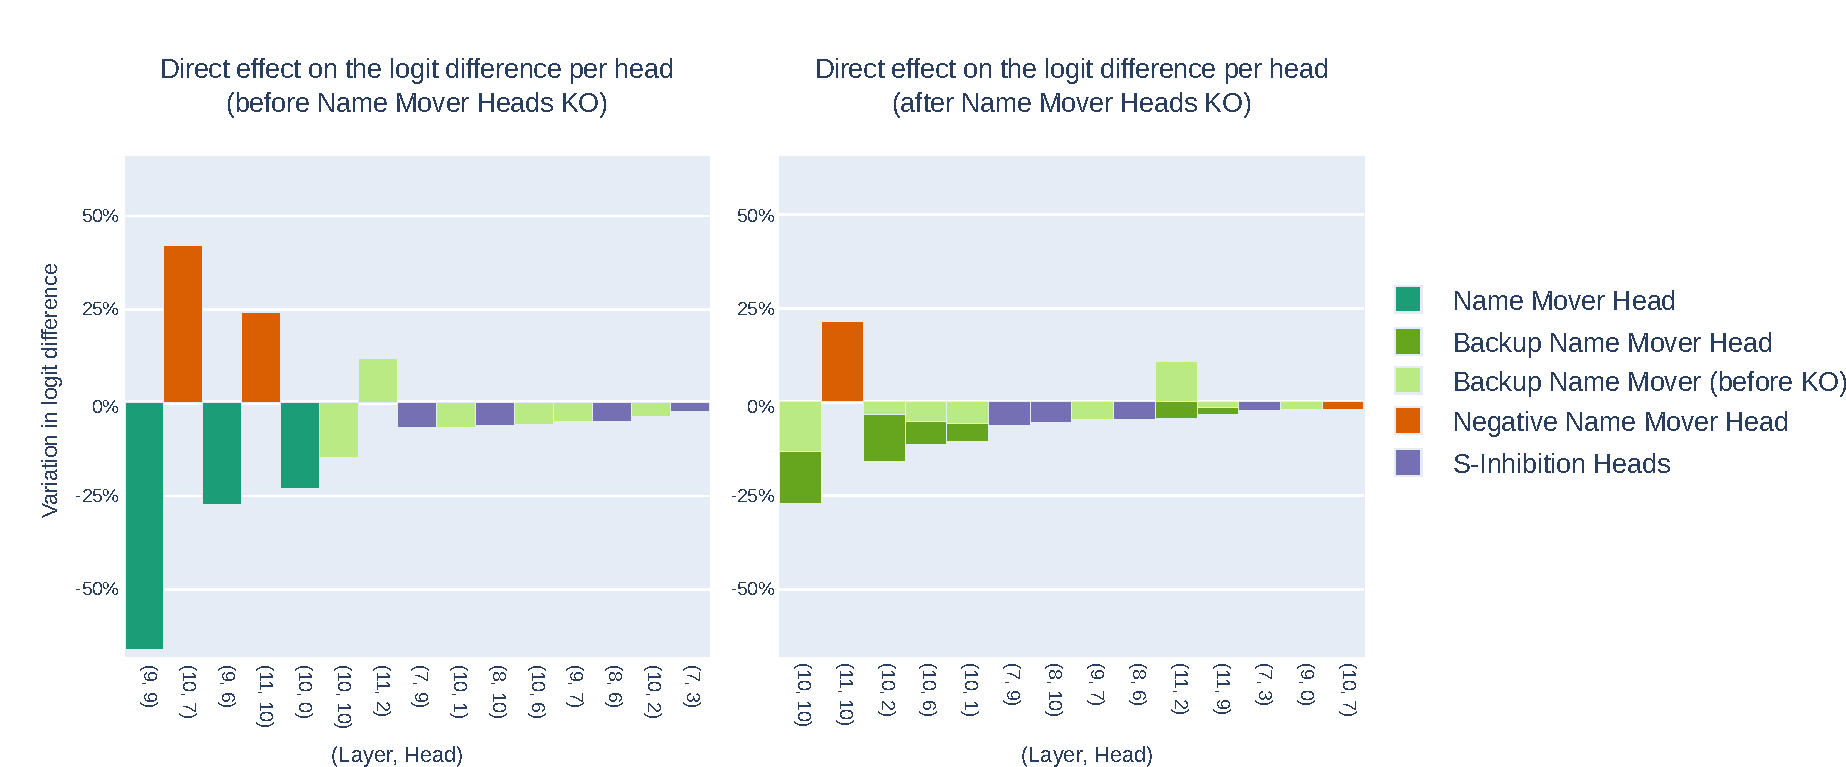
\includegraphics[width=\textwidth]{figs/backup_nm_discovery_direct_effect.pdf}
     \caption{Discovery of the Backup Name Mover Heads. Left: results from the path patching experiment in Figure \ref{fig:name_moversB}. Right: the same path patching experiment results except computed after knocking out the Name Mover Heads. In both plots, the heads are ordered by decreasing order of the absolute value of their effect.}
     \label{fig:backup_nm_discovery}
\end{figure}
 

\begin{figure}
    \centering
    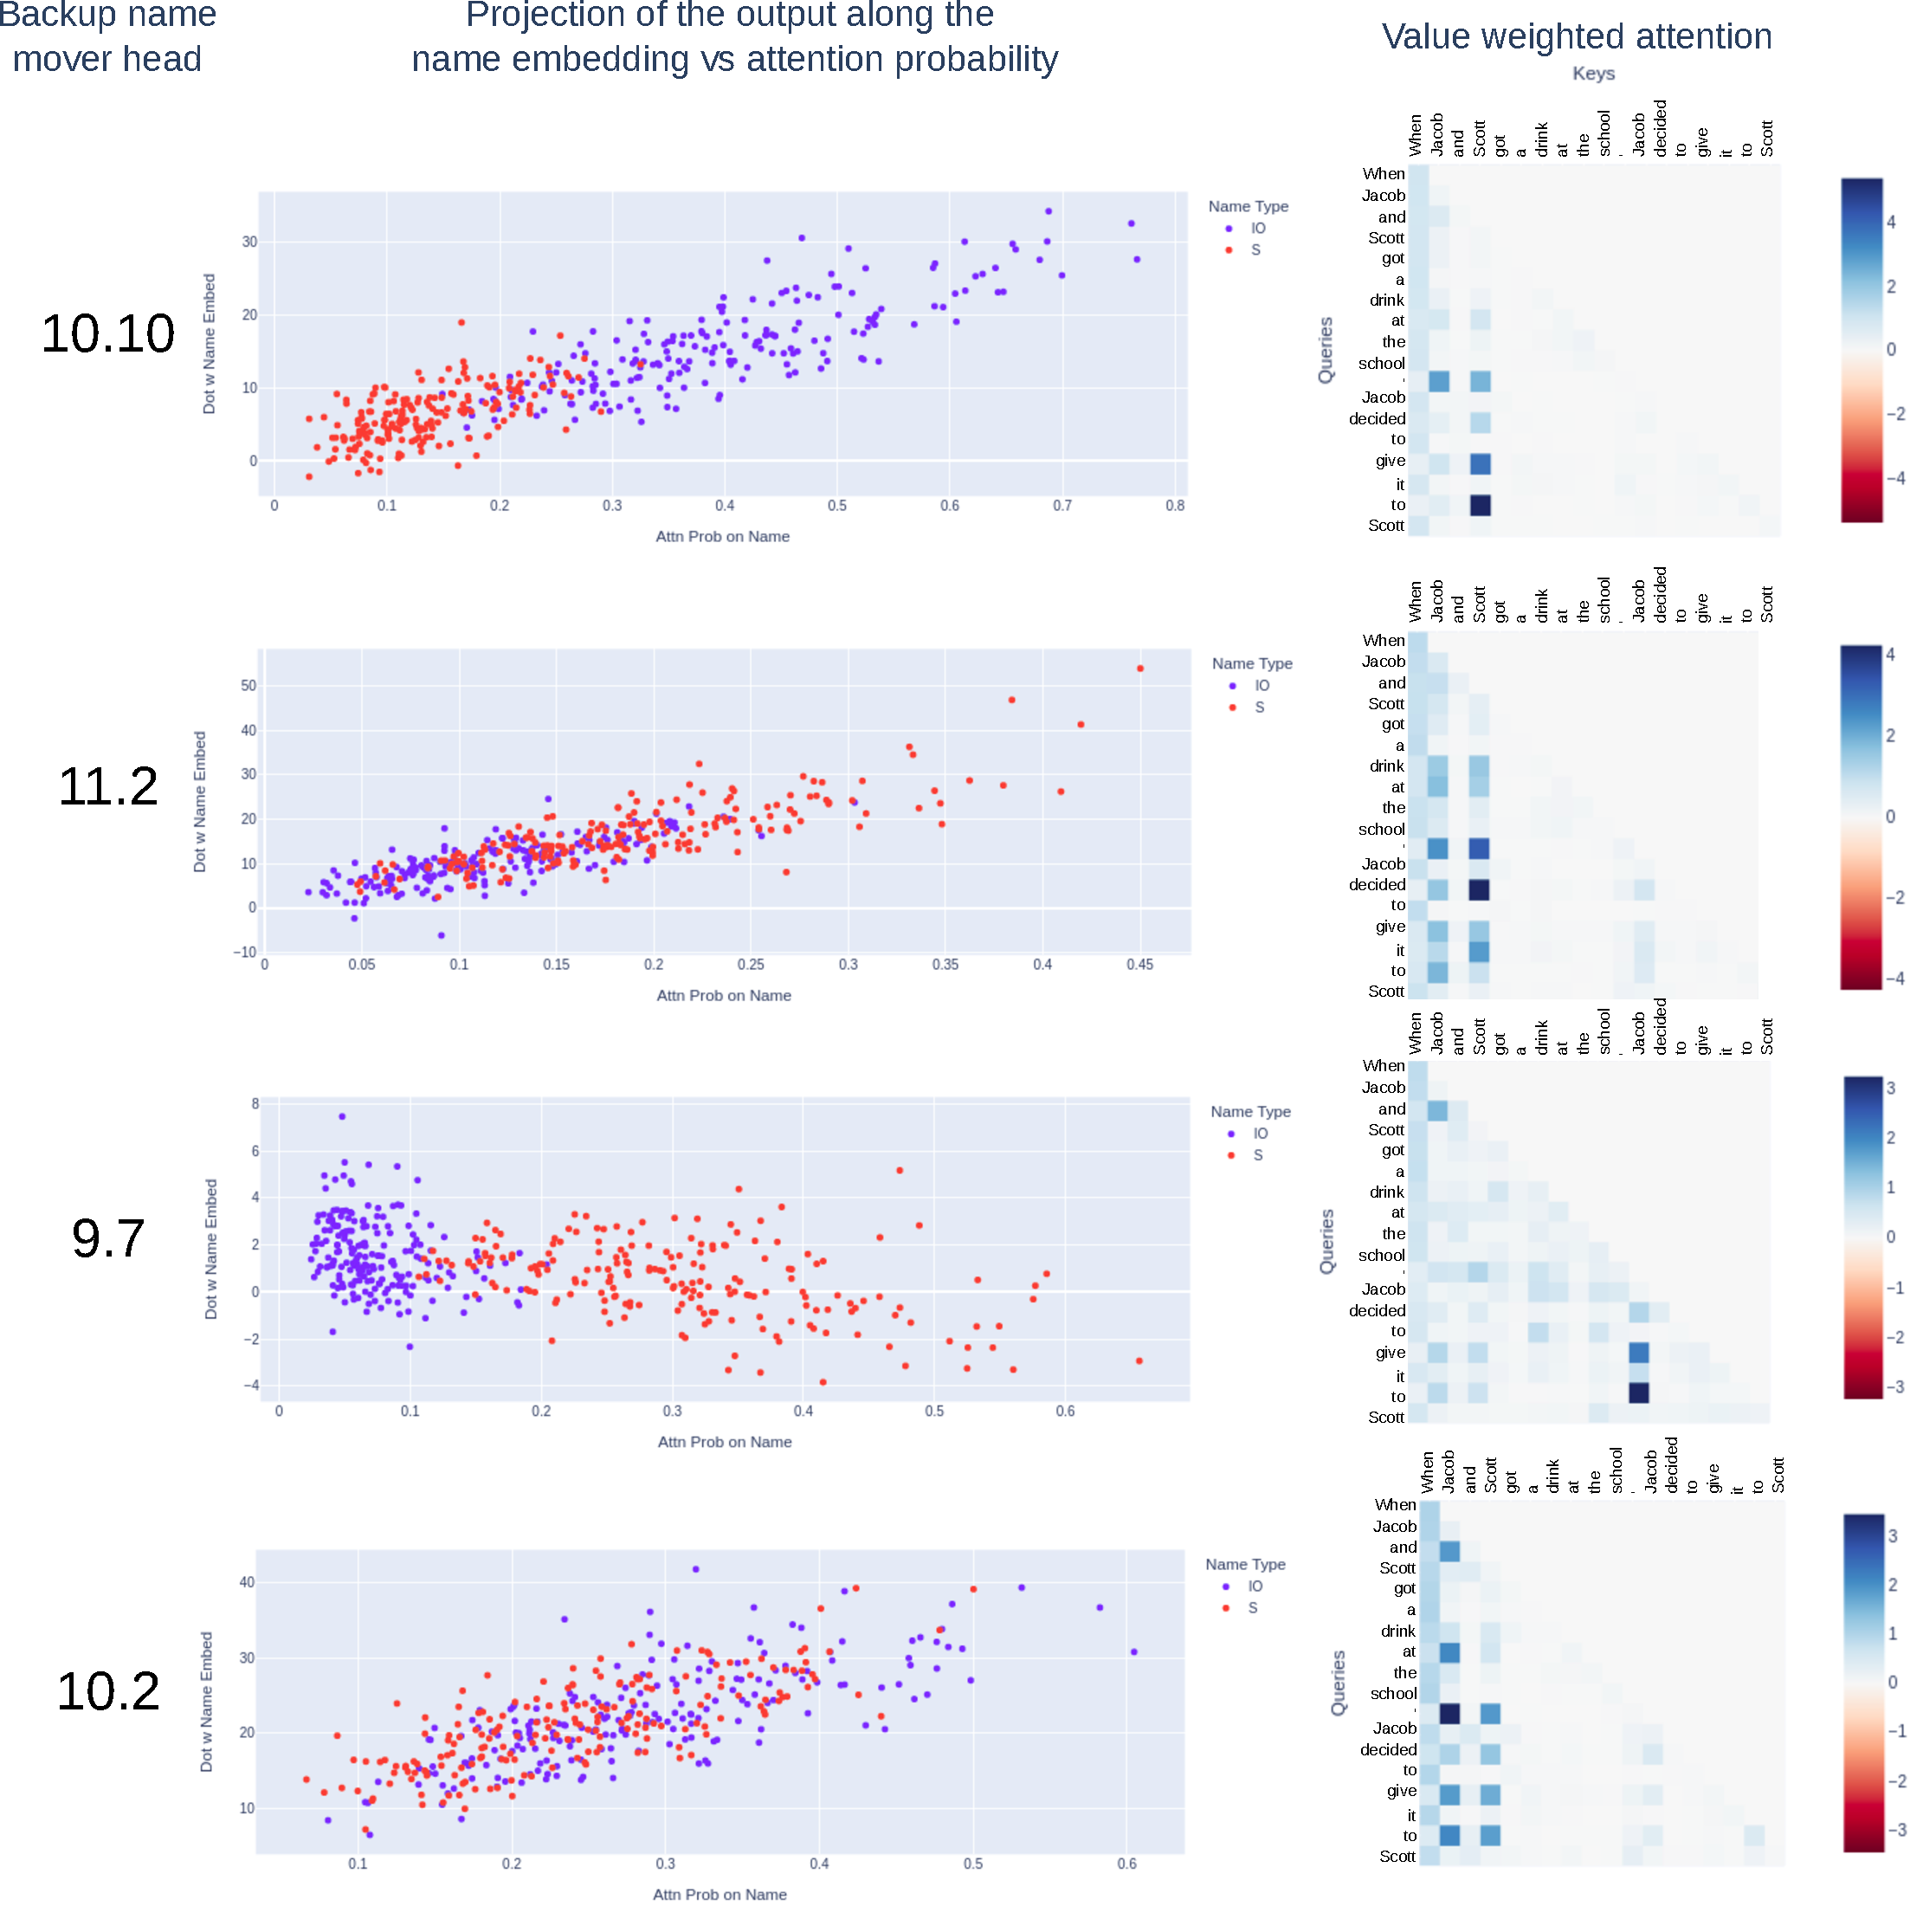
\includegraphics[width=\textwidth]{figs/backup_nm_analysis.pdf}
    \caption{Four examples of Backup Name Mover Heads. Left: attention probability vs projection of the head output along $W_U[IO]$ or $W_U[S]$ respectively. Right: Attention pattern on a sample sequence.}
    \label{fig:backup_nm_analyisis}
\end{figure}

\section{GPT-2 small full architecture} \label{app:notation}

Here we define all components of the GPT-2 architecture, including those we don't use in the main text. GPT-2 small has the following parameters

\begin{compactitem}
\item $N$: number of input tokens.
\item $V$: length of vocabulary of tokens.
\item $d$: residual stream dimension.
\item $L$: number of layers.
\item $H$: number of heads per layer.
\item $D$: hidden dimension of MLPs.
\end{compactitem}

It uses layer norm, the non-linear function

\begin{equation}
\text{LN}(x) \eqdef \frac{x-\bar{x}}{\sqrt{\sum_i (x_i - \bar{x}_i )^2}},
\label{eqn:layer_norm_definition}
\end{equation}

where the mean and the difference from the mean sum are over all components of the dimension $d$ vector in each sequence position. This is then followed by a learned linear transformation $M$ (different for each layer norm).

In GPT-2 the MLPs all have one hidden layer of dimension $D$ and use the $\text{GeLU}$ non-linearity. Their input is the layer normed state of the residual stream.

We addressed the parametrisation of each attention head in the main text, and cover the technical details of the $W_{QK}$ and $W_{OV}$ matrix here: the attention pattern is $A_{i, j} = \text{softmax}( x^T W_{QK}^{i, j} x )$ where the softmax is taken for each token position, and is unidirectional. We then have $h_{i, j}(x) \eqdef M \circ \text{LN} ( (A_{i, j} \otimes W_{OV}^{i, j}) . x)$. 
% \todo{this is complete, but therefore very dense and also repeats anthropic. Cut down???}

% GPT-2 takes as input $N$ tokens as a sequence $T$. % , that are one-hot encoded as $w \in \mathbb{R}^{N \times V}$
Algorithm \ref{gpt2_algo} describe how these elements are combined in the forward pass of GPT-2 small.

\begin{algorithm}
\caption{GPT-2.}\label{gpt2_algo}
\begin{algorithmic}[1]
\Require $\text{Input tokens $T$; returns logits for next token.}$
% \State $K \gets \emptyset$
\State $w \gets \text{One-hot embedding of T}$
\State $x_0 \gets W_E w \text{ (sum of token and position embeddings)} $
\For{$i=0$ to $L$}
    \State $y_i \gets 0 \in \mathbb{R}^{N \times d}$
    \For{$j=0$ to $H$}
        \State $y_i \gets y_i + h_{i, j}(x_i), \text{ the contribution of attention head $(i, j)$}$
    \EndFor
    \State $y_i' \gets m_i(y_i), \text{ the contribution of MLP at layer $i$}$ 
    \State $x_{i+1} \gets x_i + y_i + y_i' \text{ (update the residual stream)}$ 
\EndFor \\
\Return $W_U \circ M \circ \text{LN} \circ x_{L}$
\end{algorithmic}
\end{algorithm}


\section{Validation of the induction mechanism on sequences of random tokens} \label{app:random_tok_seq}

We run GPT-2 small on sequences of 100 tokens sampled uniformly at random from GPT-2's token vocabulary. Each sequence \texttt{A} was duplicated to form \texttt{AA}, a sequence twice as long where the first and second half are identical. On this dataset, we computed two scores from the attention patterns of the attention heads:
\begin{itemize}
    \item The \emph{previous token score}: we averaged the attention probability on the off-diagonal. This is the average attention from the token at position $i$ to position $i-1$.
    \item The \emph{induction score}: the average attention probability from $T_i$ to the token that comes after the first occurrence of $T_i$ (i.e. $T_{i-99}$)
\end{itemize} 

These two scores are depicted in Figure \ref{fig:random_token} (center and right) for all attention heads. 

\textbf{Previous Token Heads.} 4.11 and 2.2 are the two heads with the highest previous token score on sequences of random tokens. This is a strong validation of their role outside $\pioi$.

\textbf{Induction Heads.} \citet{olsson2022context} define an Induction Head according to its behavior on repeated sequences of random tokens. The attention head must demonstrate two properties. i) Prefix-matching property. The head  attends to \texttt{[B]} from the last \texttt{[A]} on pattern like \texttt{[A]\,[B]\,...\,[A]} ii) Copy property. The head contribute positively to the logit of \texttt{[B]} on the pattern \texttt{[A][B]...[A]}.

5.5 and 6.9 are among the 5 heads with the highest induction score. This validates their prefix-matching property introduced in \citet{olsson2022context}. 

To check their copy property, we computed the dot product $\langle h_i(X), W_U[B] \rangle$ between the output of the head $h_i$ on sequence $X$ and the embedding of the token \texttt{[B]} on repeated sequences of random tokens. The results are shown in Figure \ref{fig:copy_property_ind}. The two Induction Heads (5.5 and 6.9) appear in the 20 heads contributing the most to the next token prediction. Thus validating their copying property. 

We also noticed that the majority of the Negative, Backup and regular Name Mover Heads appear to write in the next token direction on repeated sequences of random tokens, and Negative Name Movers Heads contribute negatively. This suggests that these heads are involved beyond the IOI task to produce next-token prediction relying on contextual information.

\begin{figure}
    \centering
    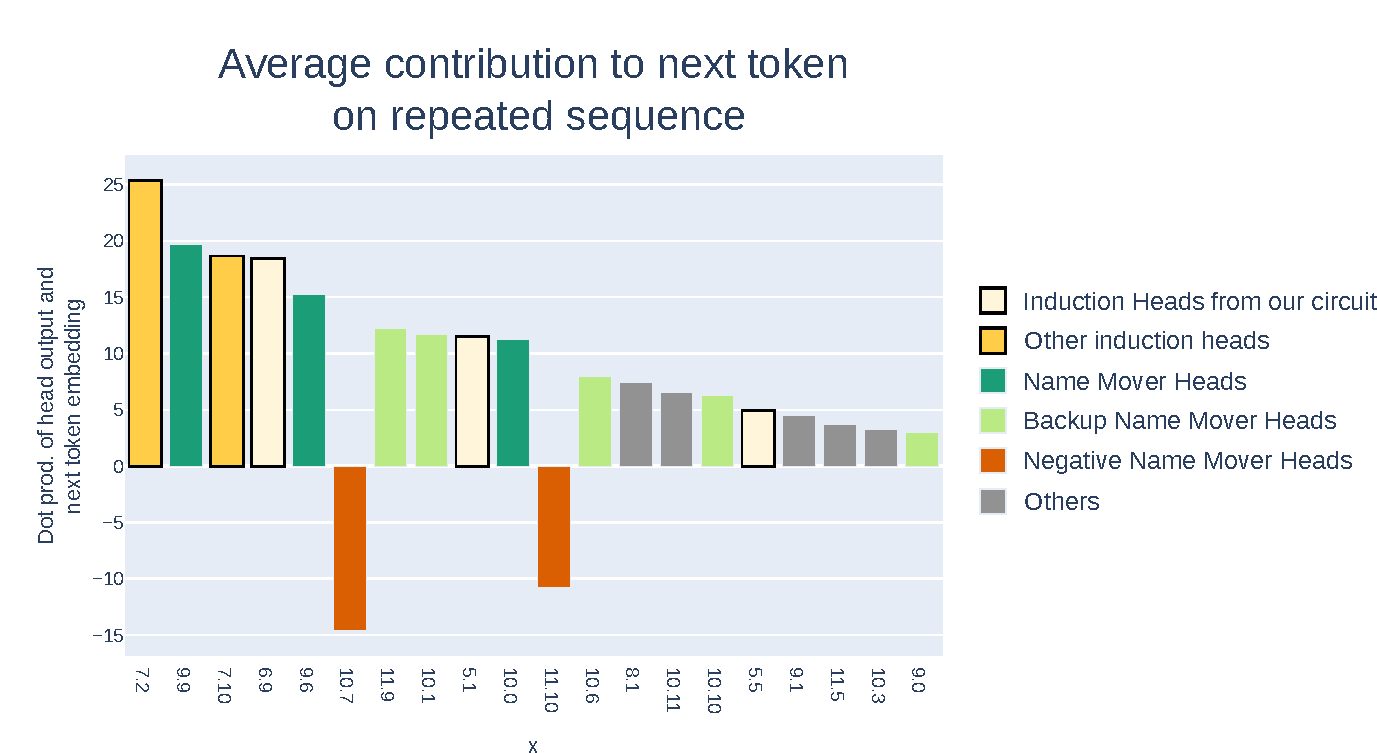
\includegraphics[width=0.9\textwidth]{figs/induct_copy_propert.pdf}
    \caption{Contribution to the next token prediction per head on repeated sequences of tokens. The heads are ordered by decreasing absolute values of contribution. Black contour: heads with attention patterns demonstrating prefix matching property. }
    \label{fig:copy_property_ind}
\end{figure}


\begin{figure}
    \centering
    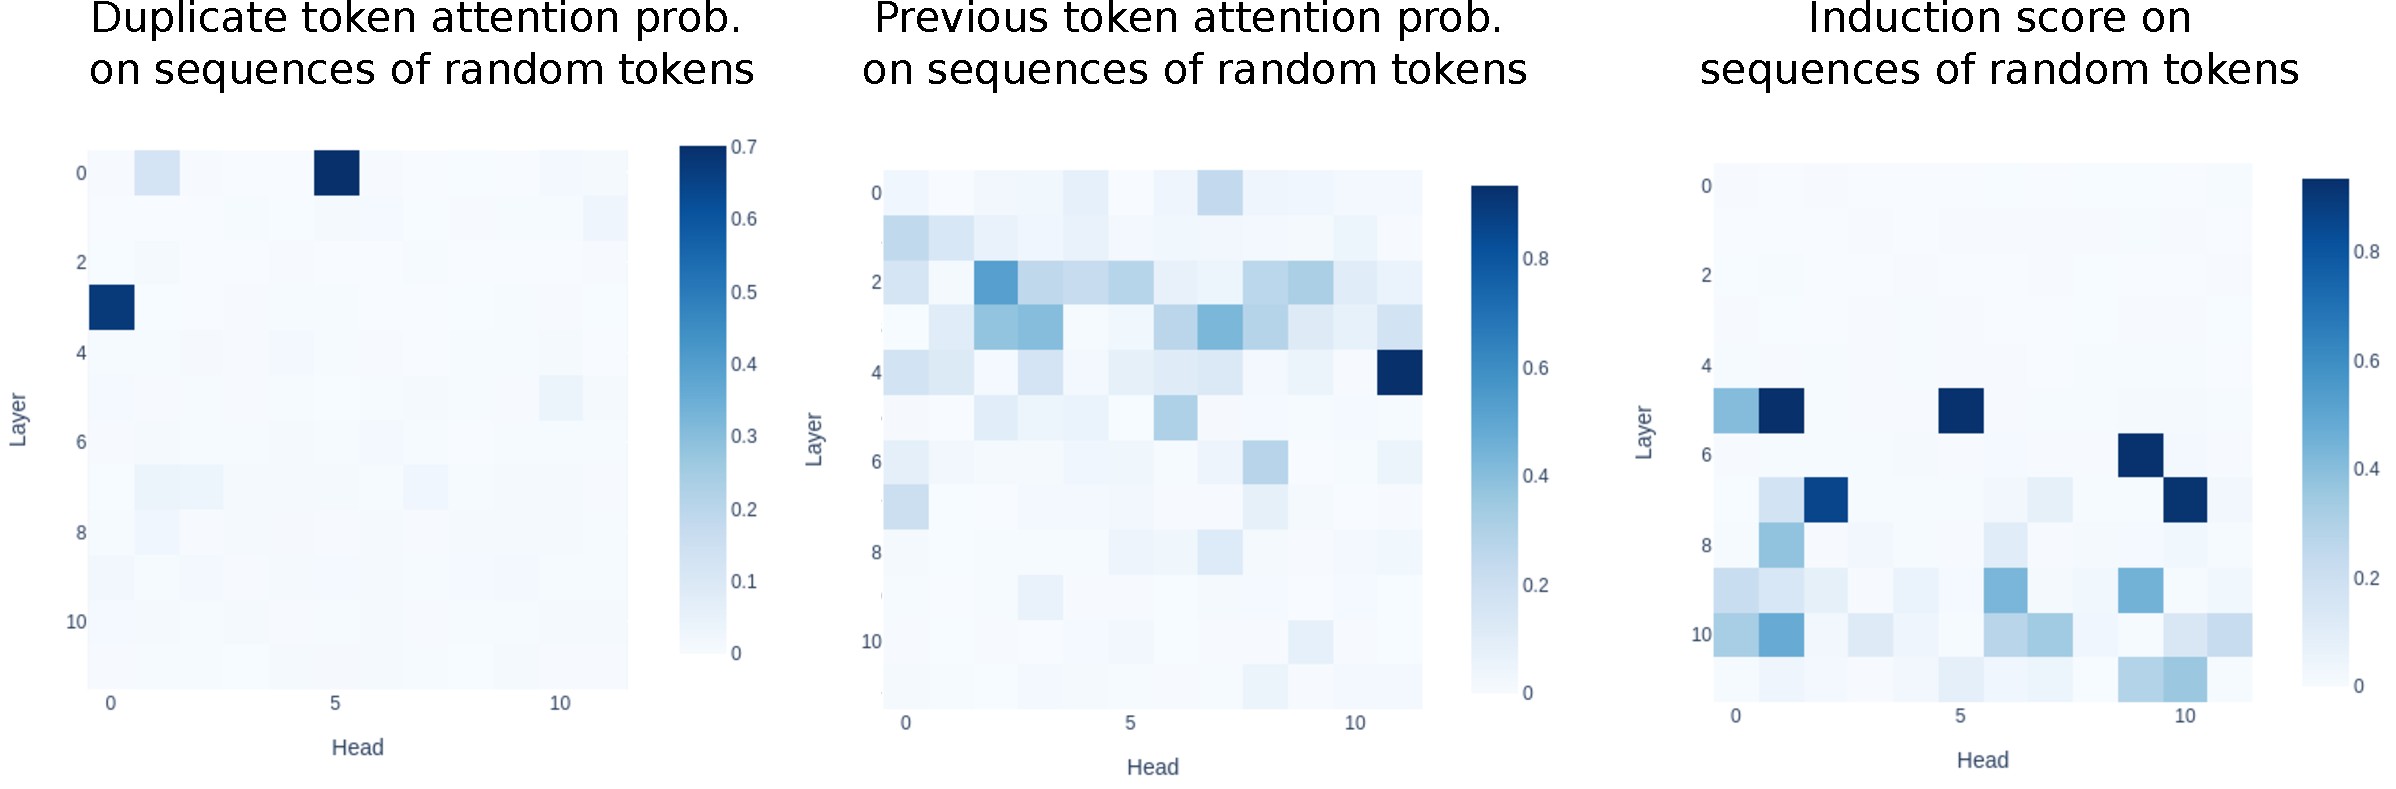
\includegraphics[width=\textwidth]{figs/random_token_seq.pdf}
    \caption{Attention scores on sequences of repeated random tokens. Left: Duplicate score, the average attention probability from a token to its previous occurrence. Center: Previous token attention score, it is the average of the off-diagonal attention probability. Right: Induction score. Average attention probability from the second occurrence of \texttt{[A]} to \texttt{[B]} on patterns \texttt{[A][B]...[A]}.}
    \label{fig:random_token}
\end{figure}

\section{Validation of Duplicate Token Heads} \label{app:validation_dups}

On the repeated sequences of random tokens (Appendix \ref{app:random_tok_seq}) we also computed the \emph{duplicate score}. For each token $T_i$ in the second half of a sequence, we average the attention probability from $T_i$ to its previous occurrence in the first half of the sequence (i.e. $T_{i-100}$). 

The duplicate token scores for all attention heads are depicted in Figure \ref{fig:random_token}. 3.0 and 0.1 are among the three heads with the highest duplicate token score (Figure \ref{fig:random_token}). This is evidence of their role of Duplicate Token Heads outside the circuit for the IOI task. 

However, the fuzzy Duplicate Head 0.10 doesn't appear on this test. By qualitatively investigating its attention patterns on Open Web Text, we found that this head attends strongly to the current token. Moreover, when the current token is a name, and it is duplicated, the head attends to its previous occurrence. 

% \section{Layer norm and the residual stream}
% \label{app:layer_norm}

% \todo{DELETE THIS SECTION IF WE END UP KEEPING IN THE DIRECT EFFECT STUFF RATHER THAN THE LOGIT LENS FOR NMS}

% The attention heads and MLPs in GPT-2 small write into the residual stream. Suppose $x$ is the final state of the residual stream after the 12 layers, at a particular sequence position. This is then converted into logits via $W_U \circ M \circ \text{LN}(x)$, where $\text{LN}$ is defined in Appendix \ref{app:notation}, $M$ is the linear transformation of the layer norm operation and $W_U$ is the unembedding matrix. 

% In order to attribute the extent to which an attention head $h_{i, j}$ writes in a direction $W_U[T]$ where $T$ is a token (always IO or S in our case), we can't simply compute $\left\langle M \circ \text{LN} \circ h_{i, j}(X), W_U[T] \right\rangle$, as the scaling factor that's used is $\sqrt{\sum_i (x_{i} - \overline{x_{i}} )^2 }$. Therefore $\overline{\text{LN}}$ in the main text uses this scaling factor:

% \begin{equation}
% \overline{\text{LN}}(h) \eqdef M \circ \frac{h - \overline{h}}{\sqrt{\sum_i (x_{i} - \overline{x_{i}} )^2 }}
% \label{eqn:ln2}
% \end{equation}

% where $h$ is the output of a head at the same sequence position as $x$.

% In order to attribute the amount which each attention head $h_i$ writes into the residual stream, suppose a head $h$ writes $x_h$ into the residual stream. Then we consider the contribution of head $h$ to the logits to be $(x_h - \overline{x_h})- / \sqrt{\sum_i (x_{12,i} - \overline{x_{12,i}} )^2 }$.

\section{Role of MLPs in the task} 
\label{app:mlp}
In the main text, all of the circuit components are attention heads. Attention heads are the only modules in transformers that move information across token positions -- a crucial component of the IOI task -- so they were our main subject of interest. However, MLPs can still play a significant role in transforming the information in each residual stream. We explored this possibility by measuring the direct and indirect effects of each of the MLPs in Figure \ref{fig:mlp_KO}. In these experiments, for each MLP in turn, we did a path patching experiment (Section \ref{sec:s_inhibition}) to measure the direct effect and a knock-out experiment for the indirect effect.

We observe that MLP0 has a significant influence on logit difference after knock-out (it reverses the sign of the logit difference) but the other layers don't seem to play a big role when individually knocked out. When all MLP layers other than the first layer are knocked out, however, the logit difference becomes $-1.1$ (a similar effect to the knockout of MLP0 alone). % We hypothesize that MLP0's output is a function of the current position only, i.e it is used primarily by the model and does not depend on earlier tokens in the context. 

\begin{figure}[H]
    \centering
    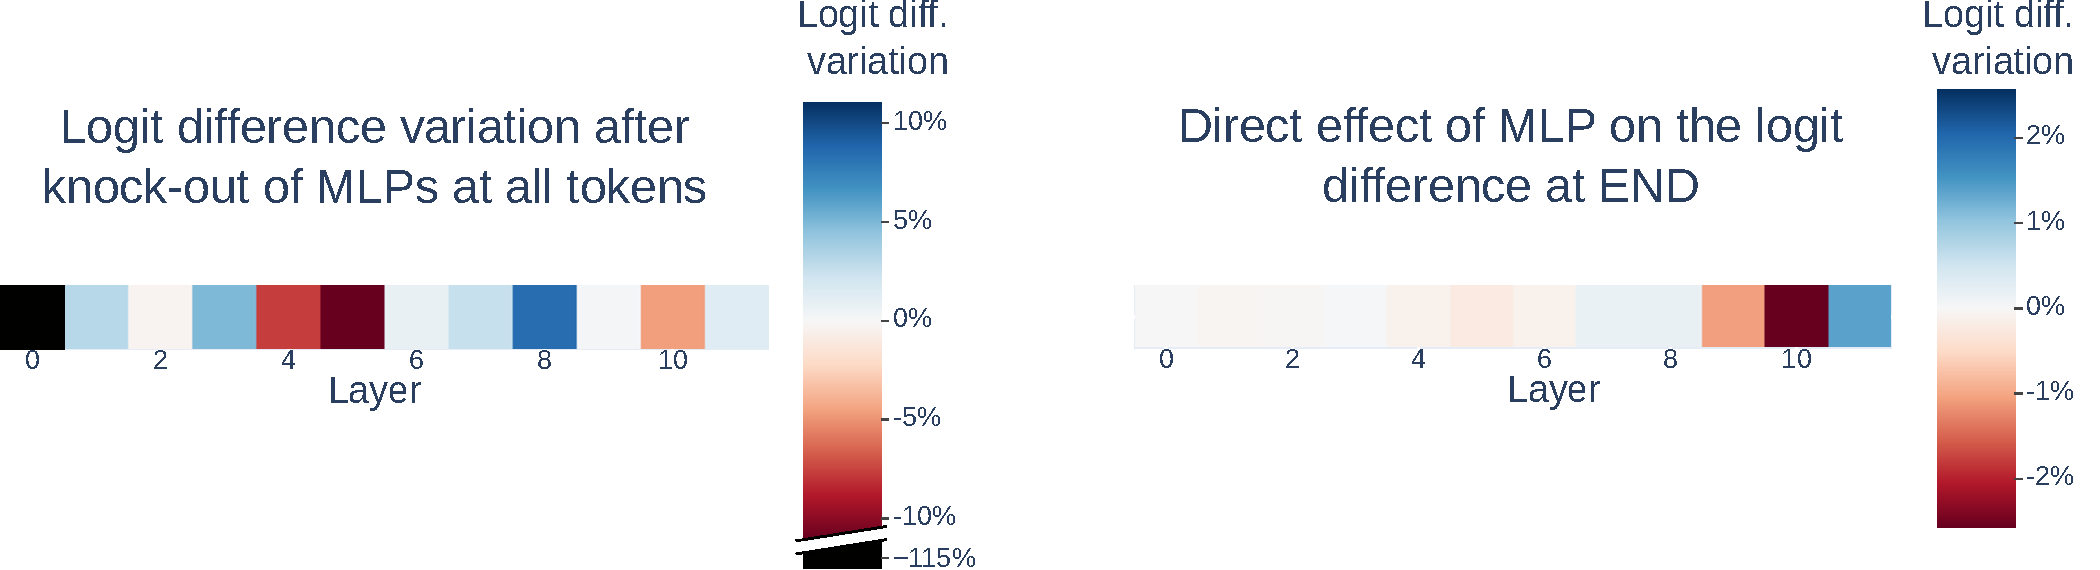
\includegraphics[width=0.9\textwidth]{figs/mlp_direct_and_indirect_effect.pdf}
    \caption{Left: change in logit difference from knocking out each MLP layer. Right: change in logit difference after a path patching experiment investigating the direct effect of MLPs on logits.}
    \label{fig:mlp_KO}
\end{figure}

\begin{comment}
\begin{figure}[H]
    \centering
    \includegraphics[width=0.8\textwidth]{figs/MLP_Writing.pdf}
    \label{fig:MLP_Writing}
    \caption{MLPs have a very small effect on writing in the IO - S direction (see scale).}
\end{figure}
\end{comment}


% \section{Trying to explain S2 Inhibition attention on S2} \label{app:S2 attention}
% \todo{}

% higher up

% In the minimality experiments, for all components $v$ we found a set $K$ such that the minimality score (Equation \ref{eqn:minimality}) was large. This table lists the sets found and the initial and final logit differences.


\section{Minimality sets} \label{app:minimality}

The sets that were found for the minimality tests are listed in Figure \ref{fig:table_minimality}.

\begin{figure}
\centering
\begin{tabular}{ |c|c|c|c|c| } 
\hline
\textbf{$v$} & Class & \textbf{$K$} $\cup \{v\}$ & $F( C \setminus (K \cup \{v\}) )$ & $F( C \setminus K )$ \\ 
\hline \hline

(9, 9) & Name Mover & [(9, 9)] & 2.26 & 2.62 \\
\hline
(10, 0) & Name Mover & [(9, 9), (10, 0)] & 1.91 & 2.26 \\
\hline
(9, 6) & Name Mover & [(9, 9), (10, 0), (9, 6)] & 2.11 & 1.91 \\
\hline
(10, 7) & Negative & [(11, 10), (10, 7)] & 4.07 & 3.13 \\
\hline
(11, 10) & Negative & [(11, 10), (10, 7)] & 4.07 & 3.27 \\
\hline
(8, 10) & S Inhibition & [(7, 9), (8, 10), (8, 6), (7, 3)] & 0.24 & 1.01 \\
\hline
(7, 9) & S Inhibition & [(7, 9), (8, 10), (8, 6), (7, 3)] & 0.24 & 0.92 \\
\hline
(8, 6) & S Inhibition & [(7, 9), (8, 10), (8, 6), (7, 3)] & 0.24 & 0.86 \\
\hline
(7, 3) & S Inhibition & [(7, 9), (8, 10), (8, 6), (7, 3)] & 0.24 & 0.43 \\
\hline
(5, 5) & Induction & [(5, 9), (5, 5), (6, 9), (5, 8)] & 0.97 & 2.12 \\
\hline
(5, 9) & Induction & [(11, 10), (10, 7), (5, 9)] & 3.33 & 4.07 \\
\hline
(6, 9) & Induction & [(5, 9), (5, 5), (6, 9), (5, 8)] & 0.97 & 1.46 \\
\hline
(5, 8) & Induction & [(11, 10), (10, 7), (5, 8)] & 3.83 & 4.07 \\
\hline
(0, 1) & Duplicate Token & [(0, 1), (0, 10), (3, 0)] & 0.60 & 1.90 \\
\hline
(0, 10) & Duplicate Token & [(0, 1), (0, 10), (3, 0)] & 0.60 & 1.66 \\
\hline
(3, 0) & Duplicate Token & [(0, 1), (0, 10), (3, 0)] & 0.60 & 1.05 \\
\hline
(4, 11) & Previous Token & [(4, 11), (2, 2)] & 1.31 & 2.28 \\
\hline
(2, 2) & Previous Token & [(4, 11), (2, 2)] & 1.31 & 1.75 \\
\hline
(11, 2) & Backup Name Mover & All previous NMs and backup NMs & 0.95 & 1.37 \\
\hline
(10, 6) & Backup Name Mover & All previous NMs and backup NMs & 1.65 & 1.88 \\
\hline
(10, 10) & Backup Name Mover & All previous NMs and backup NMs & 1.88 & 2.11 \\
\hline
(10, 2) & Backup Name Mover & All previous NMs and backup NMs & 1.49 & 1.65 \\
\hline
(9, 7) & Backup Name Mover & All previous NMs and backup NMs & 0.81 & 0.95 \\
\hline
(10, 1) & Backup Name Mover & All previous NMs and backup NMs & 1.37 & 1.49 \\
\hline
(11, 9) & Backup Name Mover & All name movers and negative heads & 0.41 & 0.45 \\
\hline
(9, 0) & Backup Name Mover & All name movers and negative heads & 0.41 & 0.45 \\
\hline

% ICLR DATA:
% (9, 6) & Name Mover & [(9, 9), (10, 0), (9, 6)] & 2.95 & 2.60 \\
% \hline
% (10, 0) & Name Mover & [(9, 9), (10, 0)] & 2.60 & 2.95 \\
% \hline
% (9, 9) & Name Mover & [(9, 9)] & 2.95 & 3.29 \\
% \hline
% (10, 7) & Negative & [(11, 10), (10, 7)] & 5.28 & 3.96 \\
% \hline
% (11, 10) & Negative & [(11, 10), (10, 7)] & 5.28 & 4.25 \\
% \hline
% (8, 10) & S Inhibition & [(7, 9), (8, 10), (8, 6), (7, 3)] & 0.39 & 1.23 \\
% \hline
% (8, 6) & S Inhibition & [(7, 9), (8, 10), (8, 6), (7, 3)] & 0.39 & 1.21 \\
% \hline
% (7, 9) & S Inhibition & [(7, 9), (8, 10), (8, 6), (7, 3)] & 0.39 & 1.17 \\
% \hline
% (7, 3) & S Inhibition & [(7, 9), (8, 10), (8, 6), (7, 3)] & 0.39 & 0.61 \\
% \hline
% (5, 5) & Induction & [(5, 5), (11, 10), (5, 8), (10, 7), (5, 9), (6, 9)] & 1.06 & 3.92 \\
% \hline
% (6, 9) & Induction & [(5, 5), (11, 10), (5, 8), (10, 7), (5, 9), (6, 9)] & 1.06 & 2.60 \\
% \hline
% (5, 9) & Induction & [(11, 10), (5, 9), (10, 7)] & 4.35 & 5.28 \\
% \hline
% (5, 8) & Induction & [(11, 10), (10, 7), (5, 8)] & 4.97 & 5.28 \\
% \hline
% (0, 1) & Duplicate Token & [(0, 1), (0, 10), (3, 0)] & 1.15 & 2.60 \\
% \hline
% (0, 10) & Duplicate Token & [(0, 1), (0, 10), (3, 0)] & 1.15 & 2.35 \\
% \hline
% (3, 0) & Duplicate Token & [(0, 1), (0, 10), (3, 0)] & 1.15 & 1.72 \\
% \hline
% (4, 11) & Previous Token & [(2, 9), (4, 11), (2, 2)] & 2.07 & 2.92 \\
% \hline
% (2, 2) & Previous Token & [(2, 9), (4, 11), (2, 2)] & 2.07 & 2.51 \\
% \hline
% (2, 9) & Previous Token & [(2, 9), (4, 11), (2, 2)] & 2.07 & 2.34 \\
% \hline
% (11, 2) & Backup Name Mover & All previous NMs and distributed NMs & 1.25 & 1.96 \\
% \hline
% (10, 6) & Backup Name Mover & All previous NMs and distributed NMs & 2.38 & 2.70 \\
% \hline
% (10, 2) & Backup Name Mover & All previous NMs and distributed NMs & 2.12 & 2.38 \\
% \hline
% (10, 10) & Backup Name Mover & All previous NMs and distributed NMs & 2.70 & 2.95 \\
% \hline
% (10, 1) & Backup Name Mover & All previous NMs and distributed NMs & 1.96 & 2.12 \\
% \hline
% (9, 7) & Backup Name Mover & All previous NMs and distributed NMs & 1.00 & 1.13 \\
% \hline
% (11, 9) & Backup Name Mover & All previous NMs and distributed NMs & 1.13 & 1.25 \\
% \hline
% (11, 3) & Backup Name Mover & All previous NMs and distributed NMs & 2.63 & 2.70 \\
% \hline
% (9, 0) & Backup Name Mover & [(9, 9), (10, 0), (9, 6), (10, 10), (11, 3)] & 0.93 & 1.00 \\
% \hline


\end{tabular}
\caption{$K$ sets for minimality for each $v$.}
\label{fig:table_minimality}
\end{figure}
% \section{Investigating the consistency across templates} \label{app:template}
% \section{Investigation of the identified heads} \label{app:outside_ioi}
% \todo{also cut?}
% \section{Investigation of OWT knockouts} \label{app:owt_knockouts}
% \todo{can we cut this???}
\section{Template for adversarial examples} \label{app:advexes_templates}
The design of adversarial examples relies on adding a duplicate IO to the sentences. To this end, we used a modification of the templates described in appendix \ref{app:templates}. We added an occurrence of [A] in the form of a natural sentence, independent of the context. The list of sentence is visible in Figure \ref{fig:template_advexes}.

\begin{figure}[H]
\centering
\begin{tabular}{ |c| } 
\hline
[A] had a good day.\\
\hline
[A] was enjoying the situation.\\
\hline
[A] was tired.\\
\hline
[A] enjoyed being with a friend.\\
\hline
[A] was an enthusiast person.\\
\hline
\end{tabular}
\caption{Templates for the natural sentences used in the generation of adversarial examples. The sentences were chosen to be independent of the context.}

\label{fig:template_advexes}
\end{figure}
\section{Greedy Algorithm} \label{app:greedy}

The Algorithm \ref{greedy_algo} describes the procedure used to sample sets for checking the completeness criteria using greedy optimization. In practice, because the naïve and the full circuit are not of the same size, we chose respectively $k=5$ and $k=10$ to ensure a similar amount of stochasticity in the process. We run the procedure 10 times and kept the 5 sets with the maximal important incompleteness score (including the intermediate $K$).

\begin{algorithm}
\caption{The greedy sampling procedure for sets to validate the completeness citeria.}\label{greedy_algo}
\begin{algorithmic}[1]
\State $K \gets \emptyset$
\For{$i$ to $N$}
    \State Sample a random subset $V \subseteq C\setminus K$ of $k$ nodes uniformly.
    \State $v_{\text{MAX}}$ $\gets$ $\argmax_{v \in V} |F(C \setminus (K \cup \{v\})) - F( C\setminus K)|$
    \State $K \gets K \cup \{v_{\text{MAX}}\}$
\EndFor \\
\Return $K$
\end{algorithmic}
\end{algorithm}

As visible in Figure \ref{fig:table_complteness} the sets found by the greedy search contain a combination of nodes from different classes. This means that it is difficult to interpret how our circuit is incomplete, as mentioned in the main text. % \ac{Changed - more accurate reflection?}
% Nonetheless, the overlap between different $K$ suggest that we are missing components from $M$ that can take the place of induction heads or S-Inhibition Heads when some Name Mover Heads are knocked-out.

\begin{figure}
\centering
\begin{tabular}{ |c| } 
\hline
$K$ found by greedy optimization \\ 
\hline \hline
(9, 9), (9, 6), (5, 8), (5, 5), (2, 2) \\
\hline
(9, 9), (11, 10), (10, 7), (8, 6), (5, 8), (4, 11) \\
\hline
(10, 7), (5, 5), (2, 2), (4, 11)\\
\hline
(9, 9), (11, 10), (10, 7), (11, 2), (3, 0), (5, 8), (2, 2) \\
\hline

\end{tabular}
\caption{4 sets $K$ found by the greedy optimization procedure on our circuit.}
\label{fig:table_complteness}
\end{figure}

% REMOVE WHOLE SECTION
% \section{Techniques Overview} 
% \label{app:techniques}

% % \todo{ideally this section would be planned and written better...}

% This work involved a variety of techniques that were required to explain model behavior. 
% % We found some of these continually useful, while others caused us repeated headaches.

% \begin{compactitem}
%     \item \textbf{Knockouts}: \\
%     We used knockouts in two different ways: knocking out singular components of models, and knocking out everything in the model except particular circuits. The former was somewhat useful, and the latter we found powerful.
%     \begin{itemize}
%         \item Knockout of single components: as an attribution method, knocking out singular components was not always as powerful as techniques such as projections, since the compensation (or backup) nature of Backup Name Mover Heads in this task allowed components to be knocked out and their true effect size masked (Figure \ref{fig:backup_nm_discovery}).
%         \item Knockouts of all components except a circuit: on the other hand, knocking out all components except a circuit enabled us to isolate behaviors in this task where behavior was sparse, and check the components of our circuit while ignoring the vast percentage of components of the network, making work manageable.
%     \end{itemize}
%     What was very important for the success of knockout experiments was the choice of reference distribution for knockout. Several early experiments that didn't use the in-template ablation on the CDE dataset gave inaccurate signal on which model components were completing which tasks. For example, mean ablations on a distribution where there is copying cause the Induction Heads and Duplicate Token heads to work as intended (as in the ACC distribution patches in Appendix \ref{app:copy} \todo{probably rewrite this as that needs be cut}), and so these ablations suggest that these components are not useful for the circuit's performance.
%     % This situation more generally exposes how delicate and important the distribution for mean-ablations is. 
    
%     % Additionally, earlier iterations of our work used `semantic knockouts' where we averaged the activations for the IO token across different template indices,\footnote{For example, one template sentence begins `After the lunch, Mary and John ...'. The IO token `Mary' appears later in the context than in the `When Mary and John ...' example.} and inserted this average in different positions. This led to strong success on some templates, and large failures on other templates, suggesting that averaging across different sequence positions leads to artifacts that are avoided with less other knockout methods. 
%     For a more general knockout the OpenWebText dataset (GPT's training data) can be used. However, we found that this led to noisier results (though our circuit components still passed the tests of significance when these ablations were used).
%     \item \textbf{Attention pattern analysis}: \\
%     Using attention patterns to explain behavior is always worrying due to the possibility that information has accumulated on that token primarily from previous tokens, or that the position with large attention paid to isn't actually writing an important value into the residual stream. In our work however, analyzing attention patterns was generally a necessary first step before further experiments could be ran, and in this small model, both of the worrying cases did not generally arise. 
%     % , a frustrating case of the information build up,
%     \item \textbf{Patching}: \\
%     Patching was an important method we used to verify causal explanations that were generally formed from correlational evidence. In this way our use case is similar to (\citet{syntactic_Agreement_Mechanisms}). We were surprised however that in general patching gave clear signal on the changes in behavior. This may be because we generally patched from inputs like the CDE distribution (which was successful in knocking out too). Therefore, keeping the context of the sentence templates may be generally useful. This could be either because the other words in the templates allow the model to realise that it should be doing IOI, or that introducing inputs from other distributions introduces noise that the model picks up on and uses, when this is not intended. 
% \end{compactitem}